% =====================================================================
% Rapport d'avancement Sprint 2 - SkillSeek AI
% Auteur : Aymen Benrbib - ESI (ISITD) - Stage BC SKILLS 2026
% Compilation : pdflatex (Overleaf : compiler "pdfLaTeX", 2 passes)
% IMPORTANT : placer le logo a cote du .tex sous le nom "bc_skills.jpg"
% =====================================================================
\documentclass[11pt,a4paper]{article}

\usepackage[utf8]{inputenc}
\usepackage[T1]{fontenc}
% Francisation : utilise babel-french s'il est installe, sinon bascule sur une
% francisation manuelle equivalente afin que le document compile partout.
\IfFileExists{french.ldf}{%
  \usepackage[french]{babel}%
}{%
  \renewcommand{\contentsname}{Table des matières}%
  \renewcommand{\figurename}{Figure}%
  \renewcommand{\tablename}{Tableau}%
}
\usepackage{lmodern}
\usepackage[margin=2.4cm]{geometry}
\usepackage{graphicx}
\usepackage{xcolor}
\usepackage{booktabs}
\usepackage{array}
\usepackage{longtable}
\usepackage{enumitem}
\usepackage{titlesec}
\usepackage{fancyhdr}
\usepackage{tikz}
\usepackage{float}
\usepackage{listings}
\usetikzlibrary{arrows.meta, positioning, shapes.geometric, fit, calc, backgrounds}
\usepackage{hyperref}

\raggedbottom

% ------------------ Couleurs ------------------
\definecolor{primaire}{HTML}{1F3A5F}
\definecolor{accent}{HTML}{2E86AB}
\definecolor{fondclair}{HTML}{EEF4F8}
\definecolor{vert}{HTML}{2E7D5B}
\definecolor{gris}{HTML}{6B7A8F}

\hypersetup{colorlinks=true, linkcolor=primaire, urlcolor=accent,
  pdftitle={Rapport d'avancement Sprint 2 - SkillSeek AI}, pdfauthor={Aymen Benrbib}}

% ------------------ Titres ------------------
\titleformat{\section}{\Large\bfseries\color{primaire}}{\thesection}{0.6em}{}
\titlespacing*{\section}{0pt}{14pt}{8pt}
\titleformat{\subsection}{\large\bfseries\color{primaire}}{\thesubsection}{0.6em}{}
\titleformat{\subsubsection}{\normalsize\bfseries\color{accent}}{\thesubsubsection}{0.6em}{}

% ------------------ En-tete / pied ------------------
\pagestyle{fancy}
\fancyhf{}
\fancyhead[L]{\small\color{primaire} Rapport d'avancement Sprint 2 -- SkillSeek AI}
\fancyhead[R]{\small\color{primaire} BC SKILLS -- 2026}
\fancyfoot[C]{\small\thepage}
\renewcommand{\headrulewidth}{0.4pt}

% ------------------ Styles TikZ ------------------
\tikzset{
  bloc/.style={rectangle, rounded corners=2pt, draw=primaire, fill=fondclair,
    text=primaire, font=\small\bfseries, minimum height=8mm,
    minimum width=22mm, align=center, inner sep=1.6mm},
  blocia/.style={bloc, draw=accent, fill=white, text=accent},
  ecran/.style={rectangle, rounded corners=2pt, draw=gris, fill=white,
    font=\scriptsize, align=center, minimum height=6.5mm, minimum width=27mm,
    inner sep=1mm},
  etat/.style={rectangle, rounded corners=4pt, draw=primaire, fill=fondclair,
    font=\scriptsize, align=center, minimum height=7mm, minimum width=20mm},
  fleche/.style={-{Stealth[length=2.2mm]}, thick, color=primaire},
  flechefine/.style={-{Stealth[length=1.8mm]}, color=gris},
  etiquette/.style={font=\scriptsize, color=primaire, align=center},
  vie/.style={dashed, color=gris}
}

\lstset{
  basicstyle=\ttfamily\scriptsize,
  backgroundcolor=\color{fondclair},
  frame=single,
  rulecolor=\color{gris},
  breaklines=true,
  keywordstyle=\color{primaire}\bfseries,
  commentstyle=\color{vert},
  showstringspaces=false,
  language=Python
}

\begin{document}

% =====================================================================
% PAGE DE GARDE
% =====================================================================
\begin{titlepage}
  \centering
  \IfFileExists{bc_skills.jpg}{%
    
\includegraphics[width=4.5cm]{bc_skills.jpg}%
  }{%
    \fbox{\parbox[c][3cm][c]{4.5cm}{\centering\small\color{gris}
      Logo BC SKILLS\\ (ajouter \texttt{bc\_skills.jpg})}}%
  }\\[1cm]
  {\color{primaire}\rule{\textwidth}{2pt}}\\[1cm]
  {\large École des Sciences de l'Information (ESI)}\\[0.2cm]
  {\normalsize Filière : Ingénierie des Systèmes d'Information et Transformation Digitale (ISITD)}\\[2cm]

  {\Huge\bfseries\color{primaire} Rapport d'avancement}\\[0.4cm]
  {\Large\bfseries\color{accent} Sprint 2}\\[0.7cm]
  {\LARGE\bfseries SkillSeek AI}\\[0.8cm]
  {\large Plateforme intelligente de gestion du recrutement\\ Interface utilisateur, parcours métier et notifications}\\[2.5cm]

  \begin{tabular}{ll}
    \textbf{Auteur :}              & Aymen Benrbib \\[2mm]
    \textbf{Organisme d'accueil :} & BC SKILLS \\
  \end{tabular}\\[2.5cm]

  {\color{primaire}\rule{\textwidth}{2pt}}
\end{titlepage}

\tableofcontents
\newpage

% =====================================================================
\section{Objet du rapport}
% =====================================================================
Ce document présente l'état d'avancement du projet \textbf{SkillSeek AI} à la clôture du Sprint~2. Il rappelle brièvement les acquis du Sprint~1, détaille les réalisations de la période, présente la conception associée à travers les diagrammes UML de référence, et expose la planification jusqu'à la livraison finale prévue le 16 août 2026.

% =====================================================================
\section{Rappel du Sprint 1}
% =====================================================================
Le Sprint~1, clôturé le 15 juillet 2026, a livré le socle technique du projet : dépôt structuré avec chaîne d'intégration continue, environnement entièrement conteneurisé (base de données et interface de programmation démarrées par une commande unique), modèle de données couvrant les sept entités du système, et couche de sécurité comprenant l'authentification par jeton, le hachage des mots de passe et un contrôle d'accès par rôles appliqué en temps réel. L'ensemble était validé par neuf tests automatisés.

Ce socle n'a nécessité aucune reprise durant le Sprint~2, ce qui confirme la pertinence des choix d'architecture initiaux.

% =====================================================================
\section{Synthèse de l'avancement}
% =====================================================================

\subsection{État global}

\begin{center}
\small
\begin{tabular}{lccp{5.4cm}}
  \toprule
  \textbf{Sprint} & \textbf{Période} & \textbf{État} & \textbf{Périmètre} \\
  \midrule
  Sprint 1 & 06/07 -- 15/07 & \textcolor{vert}{\textbf{Terminé}} & Socle technique, base de données, sécurité \\[1mm]
  Sprint 2 & 16/07 -- 27/07 & \textcolor{vert}{\textbf{Terminé}} & Interface utilisateur, parcours métier, notifications \\[1mm]
  Sprint 3 & 28/07 -- 06/08 & \textcolor{accent}{À venir} & Analyse des CV et classement automatique \\[1mm]
  Sprint 4 & 07/08 -- 16/08 & Planifié & Assistant conversationnel, décisionnel, Power BI \\
  \bottomrule
\end{tabular}
\end{center}

\vspace{2mm}
\noindent Avancement global estimé : \textbf{60\,\%} du périmètre fonctionnel. L'application est utilisable de bout en bout pour les trois profils d'utilisateurs ; seule l'analyse automatique du contenu des CV reste à implémenter.

\subsection{Tâches du Sprint 2}

\begin{center}
\small
\begin{tabular}{clp{6.6cm}c}
  \toprule
  \textbf{ID} & \textbf{Tâche} & \textbf{Livrable vérifié} & \textbf{État} \\
  \midrule
  S2-01 & Socle de l'interface & Charte visuelle, mise en page par rôle, client d'accès à l'interface de programmation & \textcolor{vert}{OK} \\
  S2-02 & Écrans d'authentification & Connexion, inscription, orientation selon le rôle & \textcolor{vert}{OK} \\
  S2-03 & Espace d'administration & Gestion des comptes, matrice de droits & \textcolor{vert}{OK} \\
  S2-04 & Gestion des offres & Publication, critères éliminatoires, ouverture/fermeture & \textcolor{vert}{OK} \\
  S2-05 & Parcours de candidature & Dépôt de document contrôlé, suivi par étapes & \textcolor{vert}{OK} \\
  S2-06 & Audit ergonomique & Application des critères de Bastien \& Scapin & \textcolor{vert}{OK} \\
  \midrule
  S2-07 & Notifications par rôle & Système événementiel persistant (hors périmètre initial) & \textcolor{vert}{OK} \\
  \bottomrule
\end{tabular}
\end{center}

\vspace{2mm}
\noindent La tâche S2-07 ne figurait pas au périmètre initial. Elle a été ajoutée en cours de sprint : l'expérimentation des écrans a montré que sans mécanisme de notification, la séparation des rôles restait invisible pour l'utilisateur, chaque profil ignorant les actions des autres.

\subsection{Indicateurs de réalisation}

\begin{center}
\begin{tabular}{lc}
  \toprule
  \textbf{Indicateur} & \textbf{Valeur} \\
  \midrule
  Écrans livrés & 16 \\
  Points d'accès de l'interface de programmation & 27 \\
  Tests automatisés (tous réussis) & 25 \\
  Analyse statique du code & sans anomalie \\
  Éléments d'interface sans action associée & 0 \\
  \bottomrule
\end{tabular}
\end{center}

% =====================================================================
\section{Conception du Sprint 2}
% =====================================================================

\subsection{Cartographie des écrans}
La figure~\ref{fig:ecrans} présente l'organisation des écrans et leur accessibilité selon le profil de l'utilisateur connecté. Chaque profil ne dispose que de la navigation correspondant à ses attributions.

\begin{figure}[H]
  \centering
  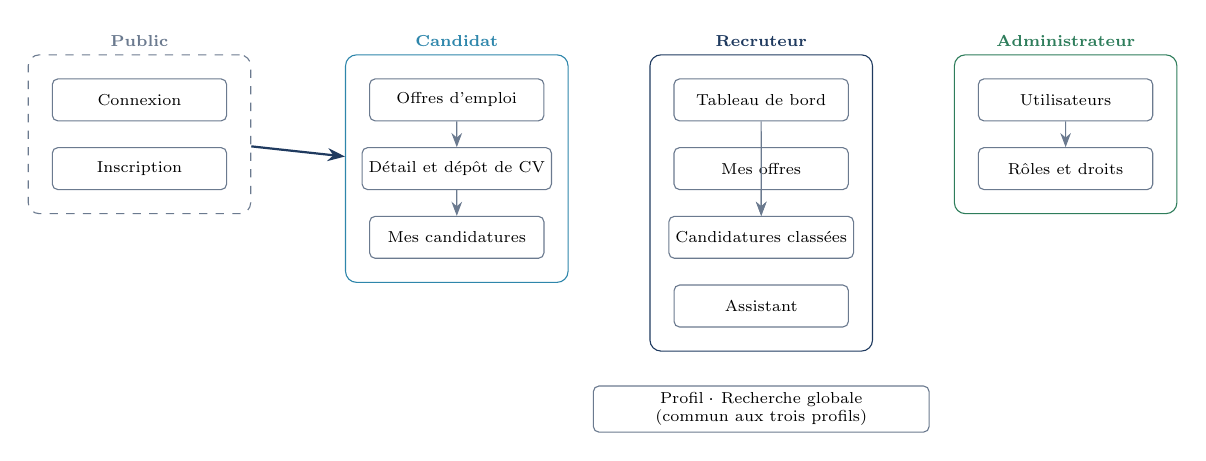
\begin{tikzpicture}[node distance=4mm and 8mm, scale=0.82, transform shape]
    % Zone publique
    \node[ecran] (co) {Connexion};
    \node[ecran, below=of co] (ins) {Inscription};
    \begin{scope}[on background layer]
      \node[draw=gris, dashed, rounded corners, fit=(co)(ins), inner sep=3mm,
            label={[font=\scriptsize\bfseries, color=gris]above:Public}] (zpub) {};
    \end{scope}

    % Candidat
    \node[ecran, right=22mm of co] (off) {Offres d'emploi};
    \node[ecran, below=of off] (det) {Détail et dépôt de CV};
    \node[ecran, below=of det] (mes) {Mes candidatures};
    \begin{scope}[on background layer]
      \node[draw=accent, rounded corners, fit=(off)(mes), inner sep=3mm,
            label={[font=\scriptsize\bfseries, color=accent]above:Candidat}] (zcan) {};
    \end{scope}

    % Recruteur
    \node[ecran, right=20mm of off] (dash) {Tableau de bord};
    \node[ecran, below=of dash] (mo) {Mes offres};
    \node[ecran, below=of mo] (cand) {Candidatures classées};
    \node[ecran, below=of cand] (ass) {Assistant};
    \begin{scope}[on background layer]
      \node[draw=primaire, rounded corners, fit=(dash)(ass), inner sep=3mm,
            label={[font=\scriptsize\bfseries, color=primaire]above:Recruteur}] (zrec) {};
    \end{scope}

    % Administrateur
    \node[ecran, right=20mm of dash] (adu) {Utilisateurs};
    \node[ecran, below=of adu] (adr) {Rôles et droits};
    \begin{scope}[on background layer]
      \node[draw=vert, rounded corners, fit=(adu)(adr), inner sep=3mm,
            label={[font=\scriptsize\bfseries, color=vert]above:Administrateur}] (zadm) {};
    \end{scope}

    % Commun aux trois profils, place sous l'ensemble
    \node[ecran, minimum width=52mm, below=9mm of ass.south, anchor=north]
      (prof) {Profil · Recherche globale\\ \scriptsize (commun aux trois profils)};

    % Orientation automatique vers l'espace du role (precisee dans la legende)
    \draw[fleche] (zpub) -- (zcan);
    \draw[flechefine] (off) -- (det);
    \draw[flechefine] (det) -- (mes);
    \draw[flechefine] (dash) -- (cand);
    \draw[flechefine] (mo) -- (cand);
    \draw[flechefine] (adu) -- (adr);
  \end{tikzpicture}
  \caption{Cartographie des écrans par profil. Après authentification, l'utilisateur est
    orienté automatiquement vers l'espace correspondant à son rôle.}
  \label{fig:ecrans}
\end{figure}

\subsection{Diagramme de séquence : dépôt et évaluation d'une candidature}
La figure~\ref{fig:seqcand} détaille le parcours d'une candidature, depuis le dépôt du document jusqu'à la notification du recruteur.

\begin{figure}[H]
  \centering
  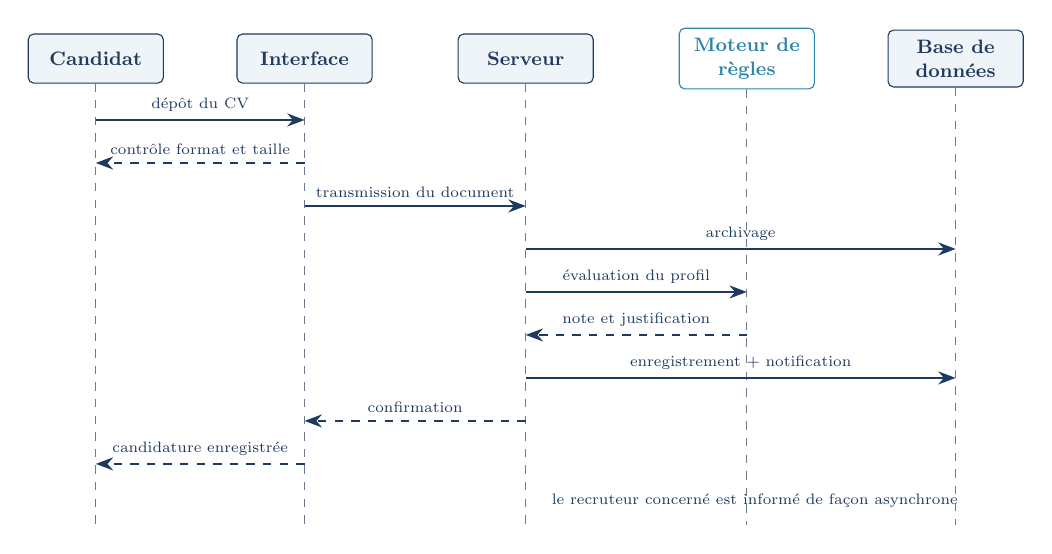
\begin{tikzpicture}[scale=0.78, transform shape]
    \node[bloc] (c) at (0, 0)     {Candidat};
    \node[bloc] (i) at (3.4, 0)   {Interface};
    \node[bloc] (a) at (7, 0)     {Serveur};
    \node[blocia] (m) at (10.6, 0) {Moteur de\\ règles};
    \node[bloc] (d) at (14, 0)    {Base de\\ données};

    \foreach \n in {c, i, a, m, d} { \draw[vie] (\n) -- ++(0, -7.6); }

    \draw[fleche] (0, -1.0) -- node[etiquette, above]{\scriptsize dépôt du CV} (3.4, -1.0);
    \draw[fleche, dashed] (3.4, -1.7) -- node[etiquette, above]{\scriptsize contrôle format et taille} (0, -1.7);
    \draw[fleche] (3.4, -2.4) -- node[etiquette, above]{\scriptsize transmission du document} (7, -2.4);
    \draw[fleche] (7, -3.1) -- node[etiquette, above]{\scriptsize archivage} (14, -3.1);
    \draw[fleche] (7, -3.8) -- node[etiquette, above]{\scriptsize évaluation du profil} (10.6, -3.8);
    \draw[fleche, dashed] (10.6, -4.5) -- node[etiquette, above]{\scriptsize note et justification} (7, -4.5);
    \draw[fleche] (7, -5.2) -- node[etiquette, above]{\scriptsize enregistrement + notification} (14, -5.2);
    \draw[fleche, dashed] (7, -5.9) -- node[etiquette, above]{\scriptsize confirmation} (3.4, -5.9);
    \draw[fleche, dashed] (3.4, -6.6) -- node[etiquette, above]{\scriptsize candidature enregistrée} (0, -6.6);
    \node[etiquette, anchor=west] at (7.3, -7.2) {\scriptsize le recruteur concerné est informé de façon asynchrone};
  \end{tikzpicture}
  \caption{Séquence de dépôt et d'évaluation d'une candidature.}
  \label{fig:seqcand}
\end{figure}

\subsection{Diagramme d'états-transitions : cycle de vie d'une candidature}
La figure~\ref{fig:etats} formalise les statuts possibles et les transitions autorisées. Chaque transition déclenche l'information du candidat concerné.

\begin{figure}[H]
  \centering
  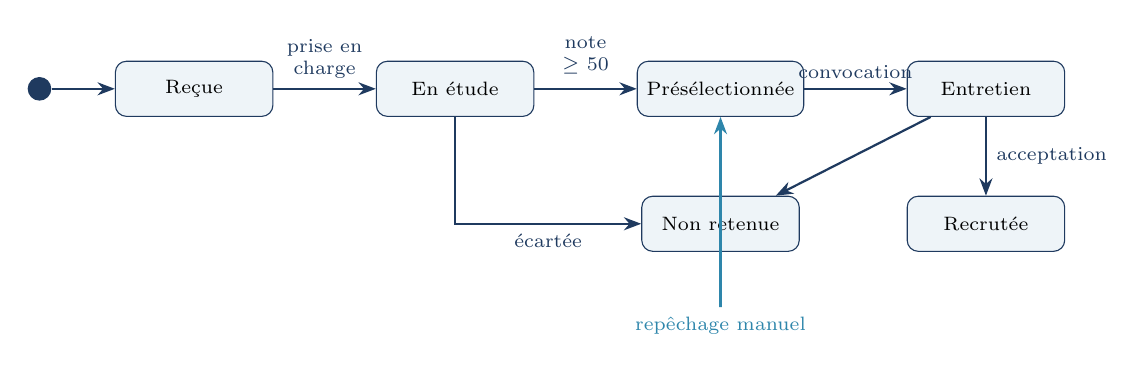
\begin{tikzpicture}[node distance=7mm and 13mm]
    \node[circle, fill=primaire, minimum size=3mm, inner sep=0] (start) {};
    \node[etat, right=8mm of start] (recue) {Reçue};
    \node[etat, right=of recue] (etude) {En étude};
    \node[etat, right=of etude] (presel) {Présélectionnée};
    \node[etat, right=of presel] (entre) {Entretien};
    \node[etat, below=10mm of entre] (recrute) {Recrutée};
    \node[etat, below=10mm of presel] (refus) {Non retenue};

    \draw[fleche] (start) -- (recue);
    \draw[fleche] (recue) -- node[etiquette, above]{\scriptsize prise en\\ \scriptsize charge} (etude);
    \draw[fleche] (etude) -- node[etiquette, above, yshift=0.5mm]{\scriptsize note\\ \scriptsize $\geq$ 50} (presel);
    \draw[fleche] (presel) -- node[etiquette, above]{\scriptsize convocation} (entre);
    \draw[fleche] (entre) -- node[etiquette, right]{\scriptsize acceptation} (recrute);
    \draw[fleche] (etude) |- node[etiquette, below, pos=0.75]{\scriptsize écartée} (refus);
    \draw[fleche] (entre) -- (refus);
    % Repechage : la decision humaine peut toujours revenir en arriere
    \draw[fleche, color=accent] (refus.south) -- ++(0,-0.7) -| node[etiquette, below, pos=0.25, color=accent]{\scriptsize repêchage manuel} (presel.south);
  \end{tikzpicture}
  \caption{États et transitions d'une candidature. Le repêchage garantit que l'humain conserve la décision finale.}
  \label{fig:etats}
\end{figure}

\subsection{Diagramme des événements de notification}
La figure~\ref{fig:notifs} présente le mécanisme retenu : chaque événement métier désigne un destinataire précis, ce qui rend la séparation des rôles perceptible par les utilisateurs.

\begin{figure}[H]
  \centering
  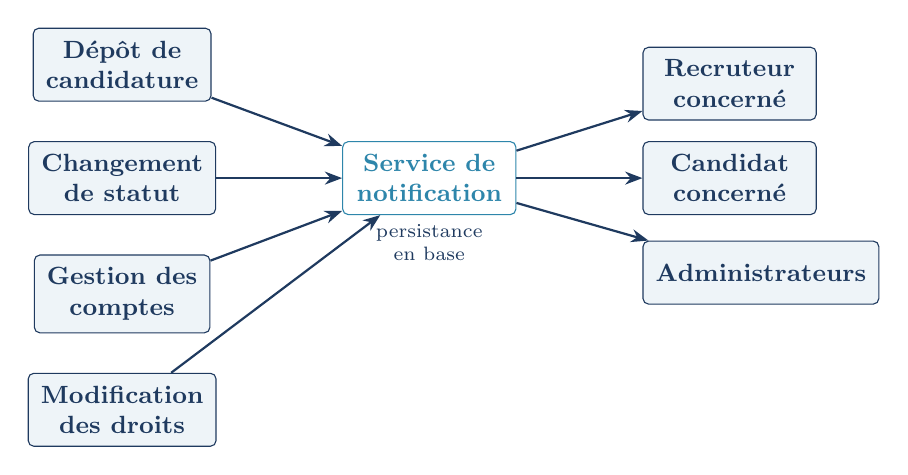
\begin{tikzpicture}[node distance=5mm and 16mm]
    \node[bloc] (ev1) {Dépôt de\\ candidature};
    \node[bloc, below=of ev1] (ev2) {Changement\\ de statut};
    \node[bloc, below=of ev2] (ev3) {Gestion des\\ comptes};
    \node[bloc, below=of ev3] (ev4) {Modification\\ des droits};

    \node[blocia, right=of ev2] (bus) {Service de\\ notification};

    \node[bloc, right=of bus, yshift=12mm] (rec) {Recruteur\\ concerné};
    \node[bloc, right=of bus] (can) {Candidat\\ concerné};
    \node[bloc, right=of bus, yshift=-12mm] (adm) {Administrateurs};

    \draw[fleche] (ev1) -- (bus);
    \draw[fleche] (ev2) -- (bus);
    \draw[fleche] (ev3) -- (bus);
    \draw[fleche] (ev4) -- (bus);
    \draw[fleche] (bus) -- (rec);
    \draw[fleche] (bus) -- (can);
    \draw[fleche] (bus) -- (adm);

    \node[etiquette, anchor=north, align=center] at (bus.south) {\scriptsize persistance\\ \scriptsize en base};
  \end{tikzpicture}
  \caption{Acheminement des notifications selon l'événement et le rôle destinataire.}
  \label{fig:notifs}
\end{figure}

% =====================================================================
\section{Réalisations du Sprint 2}
% =====================================================================

\subsection{Interface utilisateur}
Seize écrans ont été réalisés, répartis entre les trois profils d'utilisateurs et les pages communes. La charte visuelle repose sur un thème sombre déclinée en un jeu de composants réutilisables (cartes, formulaires, tableaux, panneaux latéraux, fenêtres modales, messages transitoires), garantissant une cohérence stricte d'un écran à l'autre.

Chaque écran implémente systématiquement trois états complémentaires : un état de chargement matérialisé par des zones de substitution, un état vide accompagné d'une action de sortie, et un état d'erreur proposant une nouvelle tentative. Cette discipline évite les écrans figés sans explication, principal défaut des interfaces incomplètes.

\subsection{Parcours métier}
Les trois parcours sont opérationnels de bout en bout :
\begin{itemize}[leftmargin=1.5em, nosep]
  \item \textbf{Administrateur} : création et modification des comptes, attribution des rôles, activation et désactivation, suppression avec confirmation explicite, et matrice de droits dont les modifications s'appliquent immédiatement.
  \item \textbf{Recruteur} : publication d'offres avec définition des critères éliminatoires, consultation des candidatures classées, examen détaillé d'un profil, et décision (convocation, acceptation, refus, repêchage).
  \item \textbf{Candidat} : consultation et recherche des offres, dépôt d'un document contrôlé, suivi de l'avancement de chaque candidature par étapes.
\end{itemize}

\subsection{Évaluation des candidatures}
Le moteur d'évaluation par règles métiers est opérationnel. Il combine trois composantes pondérées — correspondance des compétences, années d'expérience, niveau de diplôme — et applique en priorité les critères éliminatoires définis par offre. Toute candidature écartée par une règle conserve la trace du motif exact, présenté au recruteur en langage clair.

La règle de présélection du cahier des charges est implémentée : les candidatures dont la note est inférieure à cinquante sont écartées du classement tout en restant consultables et repêchables ; parmi les autres, les dix meilleures constituent la liste restreinte, sans remplissage artificiel lorsque leur nombre est inférieur.

\begin{lstlisting}[caption={Extrait du moteur : les critères éliminatoires sont tracés avec leur motif.}]
if offre.min_experience_years and experience < offre.min_experience_years:
    eliminatoires.append(
        f"Experience {experience} an(s) < "
        f"{offre.min_experience_years} an(s) requis"
    )
...
score = round(part_competences + part_experience + part_diplome)
if eliminatoires:
    score = min(score, 45)   # ecarte par regle metier
\end{lstlisting}

Une candidature dont le document n'a pas encore été analysé conserve une note indéterminée plutôt qu'une note nulle : elle apparaît explicitement comme \emph{en attente d'analyse}, et non comme écartée. Cette distinction évite d'imputer au candidat une insuffisance qui n'est en réalité qu'un traitement non encore effectué.

\subsection{Système de notifications}
Un mécanisme événementiel persistant a été mis en place. Chaque événement métier produit une notification adressée à un destinataire déterminé, consultable, cliquable et marquable comme lue. Le catalogue des événements est le suivant :

\begin{center}
\begin{tabular}{p{5.2cm}p{4.4cm}p{4.4cm}}
  \toprule
  \textbf{Événement} & \textbf{Destinataire} & \textbf{Finalité} \\
  \midrule
  Dépôt d'une candidature & Recruteur propriétaire de l'offre & Action attendue \\
  Changement de statut & Candidat concerné & Information sur son dossier \\
  Note élevée détectée & Recruteur & Signalement d'un profil à fort potentiel \\
  Création d'un compte & Autres administrateurs & Traçabilité \\
  Suppression d'un compte & Autres administrateurs & Traçabilité \\
  Désactivation ou réactivation & Utilisateur concerné & Explication d'un accès refusé \\
  Modification des droits & Utilisateurs du rôle et administrateurs & Transparence \\
  Publication d'une offre & Administrateurs & Suivi d'activité \\
  Échecs de connexion répétés & Administrateurs & Surveillance de sécurité \\
  Inscription d'un candidat & Candidat lui-même & Accueil et orientation \\
  \bottomrule
\end{tabular}
\end{center}

\vspace{2mm}
\noindent Le principe directeur retenu est de ne notifier que ce qui appelle une action ou ce qui serait autrement inexplicable pour l'utilisateur. Les événements sans conséquence pour le destinataire ont été volontairement exclus, afin de préserver la valeur d'attention du dispositif.

\subsection{Ergonomie et accessibilité}
L'audit prévu par le cahier des charges a été conduit selon les critères de Bastien et Scapin :
\begin{itemize}[leftmargin=1.5em, nosep]
  \item \textbf{Guidage} : intitulé explicite pour chaque champ, fil d'Ariane sur les écrans profonds, indication de l'élément de navigation actif, et retour immédiat après chaque action.
  \item \textbf{Concision} : écrans limités à l'essentiel, informations secondaires reportées dans un panneau latéral consultable à la demande.
  \item \textbf{Gestion des erreurs} : messages formulés en langage courant et positionnés au niveau du champ concerné, validation au fil de la saisie, confirmation explicite avant toute action irréversible, et possibilité d'annuler pendant cinq secondes les actions réversibles.
  \item \textbf{Accessibilité} : navigation complète au clavier avec indicateur de focus, zones cliquables dimensionnées pour un usage confortable, et libellés accessibles sur les commandes représentées par une icône.
\end{itemize}

\subsection{Vérification}
La couverture de tests a été portée de neuf à vingt-cinq cas, tous réussis. Les ajouts du Sprint~2 portent sur le moteur d'évaluation (profil conforme, insuffisance d'expérience, insuffisance de diplôme, compétences manquantes, application du seuil et du plafond), la gestion des offres et des droits associés, le tableau de bord, la modification du profil, et le cloisonnement des notifications entre utilisateurs.

\begin{center}
\begin{tabular}{lcc}
  \toprule
  \textbf{Domaine testé} & \textbf{Cas} & \textbf{Résultat} \\
  \midrule
  Authentification et sessions & 6 & \textcolor{vert}{Réussis} \\
  Contrôle d'accès & 3 & \textcolor{vert}{Réussis} \\
  Moteur d'évaluation et règle de présélection & 6 & \textcolor{vert}{Réussis} \\
  Offres, tableau de bord, profil & 5 & \textcolor{vert}{Réussis} \\
  Notifications et cloisonnement & 5 & \textcolor{vert}{Réussis} \\
  \midrule
  \textbf{Total} & \textbf{25} & \textcolor{vert}{\textbf{100 \%}} \\
  \bottomrule
\end{tabular}
\end{center}

% =====================================================================
\section{Difficultés rencontrées et corrections}
% =====================================================================
Trois difficultés méritent d'être signalées, chacune ayant conduit à une correction de conception plutôt qu'à un simple correctif technique.

\textbf{Représentation d'une candidature non évaluée.} L'attribution d'une note nulle par défaut classait les candidatures récentes parmi les profils écartés, alors que leur document n'avait simplement pas encore été traité. La note indéterminée a été introduite comme état distinct, avec un onglet dédié dans l'interface.

\textbf{Consultation des documents protégés.} L'ouverture directe d'un document dans un nouvel onglet ne transmettait pas le jeton d'authentification, rendant le fichier inaccessible. La récupération se fait désormais par le client applicatif, qui transmet l'identification puis présente le document.

\textbf{Visibilité de la séparation des rôles.} Les premiers essais ont montré que les cloisonnements entre profils, bien qu'appliqués côté serveur, restaient imperceptibles à l'usage. Le système de notifications a été ajouté pour rendre cette séparation manifeste : chaque utilisateur constate qu'il reçoit précisément ce qui relève de ses attributions.

% =====================================================================
\section{Planification}
% =====================================================================
Le stage a débuté le 6 juillet 2026 et la livraison finale est fixée au 16 août 2026. Les deux sprints réalisés respectent le calendrier prévu.

\begin{center}
\begin{tabular}{clcc}
  \toprule
  \textbf{Sprint} & \textbf{Contenu} & \textbf{Période} & \textbf{Durée} \\
  \midrule
  1 & Socle technique, base de données, sécurité & 06/07 -- 15/07 & 10 jours \\
  2 & Interface, parcours métier, notifications & 16/07 -- 27/07 & 12 jours \\
  3 & Analyse des CV, extraction, classement & 28/07 -- 06/08 & 10 jours \\
  4 & Assistant conversationnel, décisionnel, Power BI & 07/08 -- 16/08 & 10 jours \\
  \bottomrule
\end{tabular}
\end{center}

\begin{figure}[H]
  \centering
  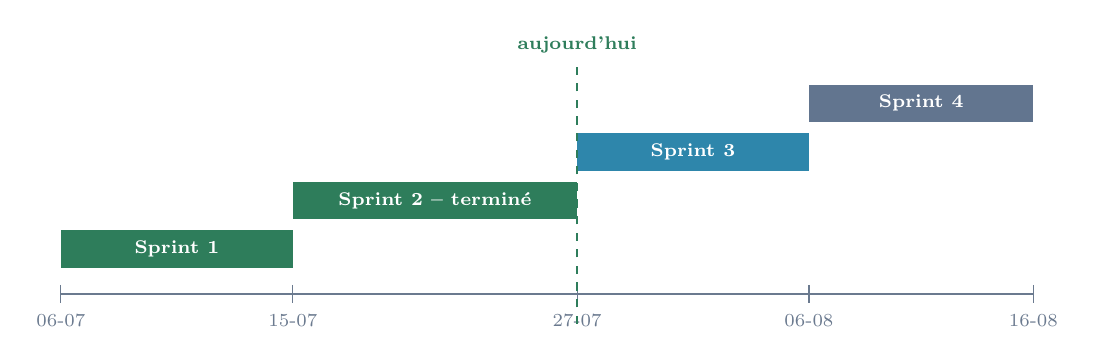
\begin{tikzpicture}[scale=0.95, transform shape]
    \draw[gris, thick] (0,0) -- (13,0);
    \foreach \x/\lab in {0/06-07, 3.1/15-07, 6.9/27-07, 10/06-08, 13/16-08} {
      \draw[gris] (\x, 0.12) -- (\x, -0.12);
      \node[font=\scriptsize, color=gris, below] at (\x, -0.15) {\lab};
    }
    \fill[vert] (0, 0.35) rectangle (3.1, 0.85);
    \node[white, font=\scriptsize\bfseries] at (1.55, 0.6) {Sprint 1};
    \fill[vert] (3.1, 1.0) rectangle (6.9, 1.5);
    \node[white, font=\scriptsize\bfseries] at (5.0, 1.25) {Sprint 2 -- terminé};
    \fill[accent] (6.9, 1.65) rectangle (10, 2.15);
    \node[white, font=\scriptsize\bfseries] at (8.45, 1.9) {Sprint 3};
    \fill[primaire!70] (10, 2.3) rectangle (13, 2.8);
    \node[white, font=\scriptsize\bfseries] at (11.5, 2.55) {Sprint 4};
    \draw[dashed, thick, color=vert] (6.9, -0.4) -- (6.9, 3.1);
    \node[font=\scriptsize\bfseries, color=vert, above] at (6.9, 3.1) {aujourd'hui};
  \end{tikzpicture}
  \caption{Avancement du projet au 27 juillet 2026.}
  \label{fig:gantt2}
\end{figure}

\subsection{Contenu du Sprint 3}
Les travaux à venir portent sur le cœur analytique du projet :
\begin{itemize}[leftmargin=1.5em, nosep]
  \item extraction du texte des documents déposés, avec reconnaissance optique en solution de repli pour les documents numérisés ;
  \item repérage automatique des compétences, du niveau de diplôme et des années d'expérience ;
  \item calcul de proximité sémantique entre le profil extrait et le descriptif de l'offre ;
  \item constitution du corpus d'apprentissage, entraînement du modèle de classification et mesure des indicateurs de performance ;
  \item vérification de l'absence de corrélation entre les notes attribuées et des attributs non pertinents.
\end{itemize}

\noindent L'architecture du Sprint~2 a été conçue pour absorber ces travaux sans reprise : le point d'accès d'évaluation et l'interface d'explication de la note existent déjà et seront simplement alimentés par les données extraites automatiquement, en remplacement de la saisie assistée actuelle.

% =====================================================================
\section{Risques et mesures}
% =====================================================================

\begin{center}
\begin{tabular}{p{4.6cm}cp{7.4cm}}
  \toprule
  \textbf{Risque} & \textbf{Criticité} & \textbf{Mesure retenue} \\
  \midrule
  Constitution du corpus d'apprentissage & Élevée & Solution de repli : classement fondé sur la proximité sémantique seule, sans apprentissage supervisé, si le corpus s'avère insuffisant. \\[1mm]
  Qualité variable des documents déposés & Moyenne & Extraction directe en premier choix, reconnaissance optique en solution de repli, et signalement explicite au recruteur en cas d'échec. \\[1mm]
  Densité du Sprint 4 & Moyenne & Priorisation : le décisionnel et le classement priment sur la mise en ligne distante, remplaçable par une démonstration conteneurisée locale. \\[1mm]
  Coût des services externes & Faible & Sélection exclusive d'outils gratuits ou en licence libre pour l'ensemble de la chaîne. \\
  \bottomrule
\end{tabular}
\end{center}

% =====================================================================
\section{Conclusion}
% =====================================================================
Le Sprint~2 est clôturé conformément au calendrier. L'application est désormais utilisable de bout en bout : un administrateur gère les comptes et les droits, un recruteur publie une offre et traite les candidatures reçues, un candidat postule et suit l'avancement de son dossier. Le mécanisme d'évaluation par règles est opérationnel et explicable, et le système de notifications rend perceptible la séparation des attributions entre profils.

L'ajout non prévu du dispositif de notifications s'est révélé déterminant pour la qualité d'usage. Il illustre l'intérêt d'une démarche itérative : l'expérimentation effective des écrans a révélé un besoin que la seule spécification n'avait pas fait apparaître.

Le projet aborde le Sprint~3 dans des conditions favorables, l'architecture ayant été préparée pour recevoir le module d'analyse automatique sans remise en cause des développements réalisés.

\end{document}
